%============================ 4. RESULTS ======================================
\isec{\faFlask}{Results of the 10 Trials}
\label{sec:results}

All 10 trials started from the same marks at 1.20\,m, ended with the normal stop
(\textit{EKF distance $\le$ 0.50\,m}, no safety stop) and lasted about 7.3\,s of driving. For each trial the robot
logged its final estimate $d_{est}$ with its uncertainty $\sigma_{EKF}$, and the distance was then measured with a tape
from the same reference point. The camera-only and wheels-only distances, logged in the same run, are listed for the
discussion.

\begin{table}[H]
\centering\small
\setlength{\tabcolsep}{5pt}
\rowcolors{2}{kfupmlight}{white}
\begin{tabular}{@{}crrrrr|rr|rr@{}}
\rowcolor{kfupm}\hd{Trial} & \hd{$d_{est}$ (m)} & \hd{$\sigma_{EKF}$ (cm)} & \hd{$d_{meas}$ (m)} & \hd{$e$ (cm)} & \hd{$|e|$ (cm)} &
  \hd{$e_{cam}$} & \hd{$e_{wheels}$} & \hd{glitches} & \hd{fixes (rej.)}\\
1  & 0.4968 & 0.88 & 0.492 & $+0.48$ & 0.48 & $+0.40$ & $+0.32$ & 0 & 196 (0)\\
2  & 0.4966 & 0.88 & 0.498 & $-0.14$ & 0.14 & $-0.16$ & $+0.76$ & 0 & 187 (0)\\
3  & 0.4948 & 0.96 & 0.495 & $-0.02$ & 0.02 & $-0.03$ & $-0.08$ & 0 & 184 (0)\\
4  & 0.4956 & 0.89 & 0.498 & $-0.24$ & 0.24 & $-0.25$ & $+0.09$ & 0 & 190 (0)\\
5  & 0.4802 & 0.88 & 0.485 & $-0.48$ & 0.48 & $-0.52$ & $-0.23$ & 0 & 203 (0)\\
6  & 0.4837 & 0.88 & 0.488 & $-0.43$ & 0.43 & $-0.54$ & $+5.81$ & 4 & 176 (0)\\
7  & 0.4774 & 0.88 & 0.480 & $-0.26$ & 0.26 & $-0.32$ & $-0.50$ & 0 & 190 (0)\\
8  & 0.4859 & 0.88 & 0.482 & $+0.39$ & 0.39 & $+0.24$ & $+4.82$ & 2 & 181 (0)\\
9  & 0.4953 & 0.95 & 0.495 & $+0.03$ & 0.03 & $-0.14$ & $+2.90$ & 2 & 205 (8)\\
10 & 0.4929 & 0.96 & 0.496 & $-0.31$ & 0.31 & $-0.30$ & $+4.25$ & 2 & 168 (0)\\
\midrule
\multicolumn{4}{r}{\textbf{MAE}} & \multicolumn{2}{r|}{\textbf{0.28\,cm}} & 0.29 & 1.98 & & \\
\multicolumn{4}{r}{\textbf{Range of errors}} & \multicolumn{2}{r|}{\textbf{0.96\,cm}} & 0.95 & 6.31 & & \\
\end{tabular}
\caption{Final distance in every trial. $e = d_{est}-d_{meas}$ is the graded error. $e_{cam}$: last camera reading
alone; $e_{wheels}$: wheel odometry alone, never corrected (both in cm, same runs). ``Glitches'': odometry steps
skipped by the guard; ``fixes'': camera corrections used (rejected by the gate). Generated from
\code{results/summary_table.csv}.}
\label{tab:trials}
\end{table}

\begin{center}
\begin{minipage}{\linewidth}
\stat[kfupm]{\faBullseye}{0.28\,cm}{mean absolute error}\hfill
\stat[accblue]{\faArrowsAltH}{0.96\,cm}{range, $-0.48$ to $+0.48$}\hfill
\stat[accpurple]{\faBalanceScale}{$-0.10$\,cm}{bias $\bar e$ (p = 0.36)}\hfill
\stat[accorange]{\faChartArea}{0.32\,cm}{std.\ deviation $\sigma$}
\end{minipage}
\end{center}

%-----------------------------------------------------------------------------
\isub{\faBullseye}{The scatter plot: estimate against tape}
\begin{figure}[H]
\centering
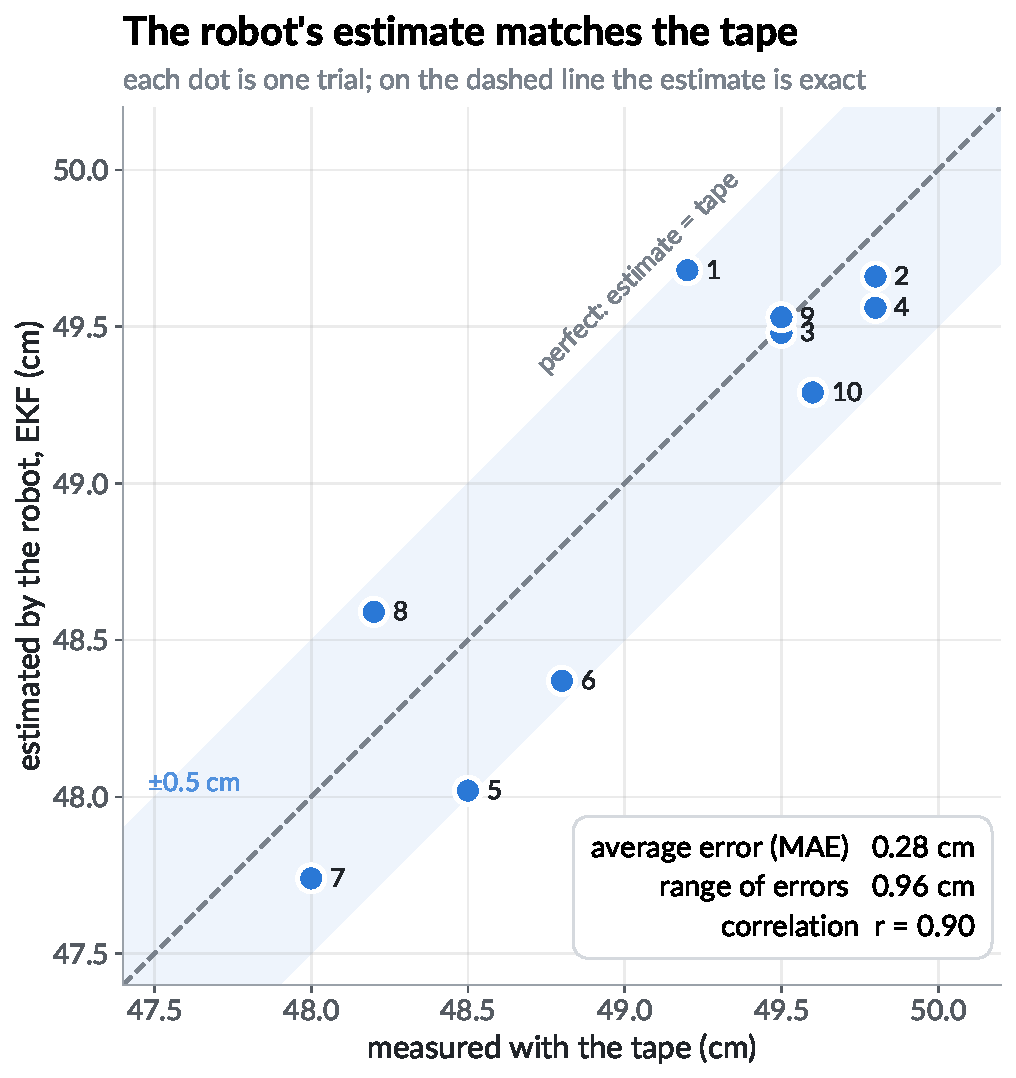
\includegraphics[width=0.66\linewidth]{figures/simple_1_scatter.pdf}
\caption{Estimated versus measured final distance, one dot per trial.
\textbf{How to read it:} on the dashed line the estimate equals the tape; the shaded band is $\pm$0.5\,cm.
All ten dots are inside the band, and they follow the line even though the robot stopped at different places
(47.8 to 49.8\,cm) because it coasted after braking.}
\label{fig:scatter}
\end{figure}

\begin{figure}[H]
\centering
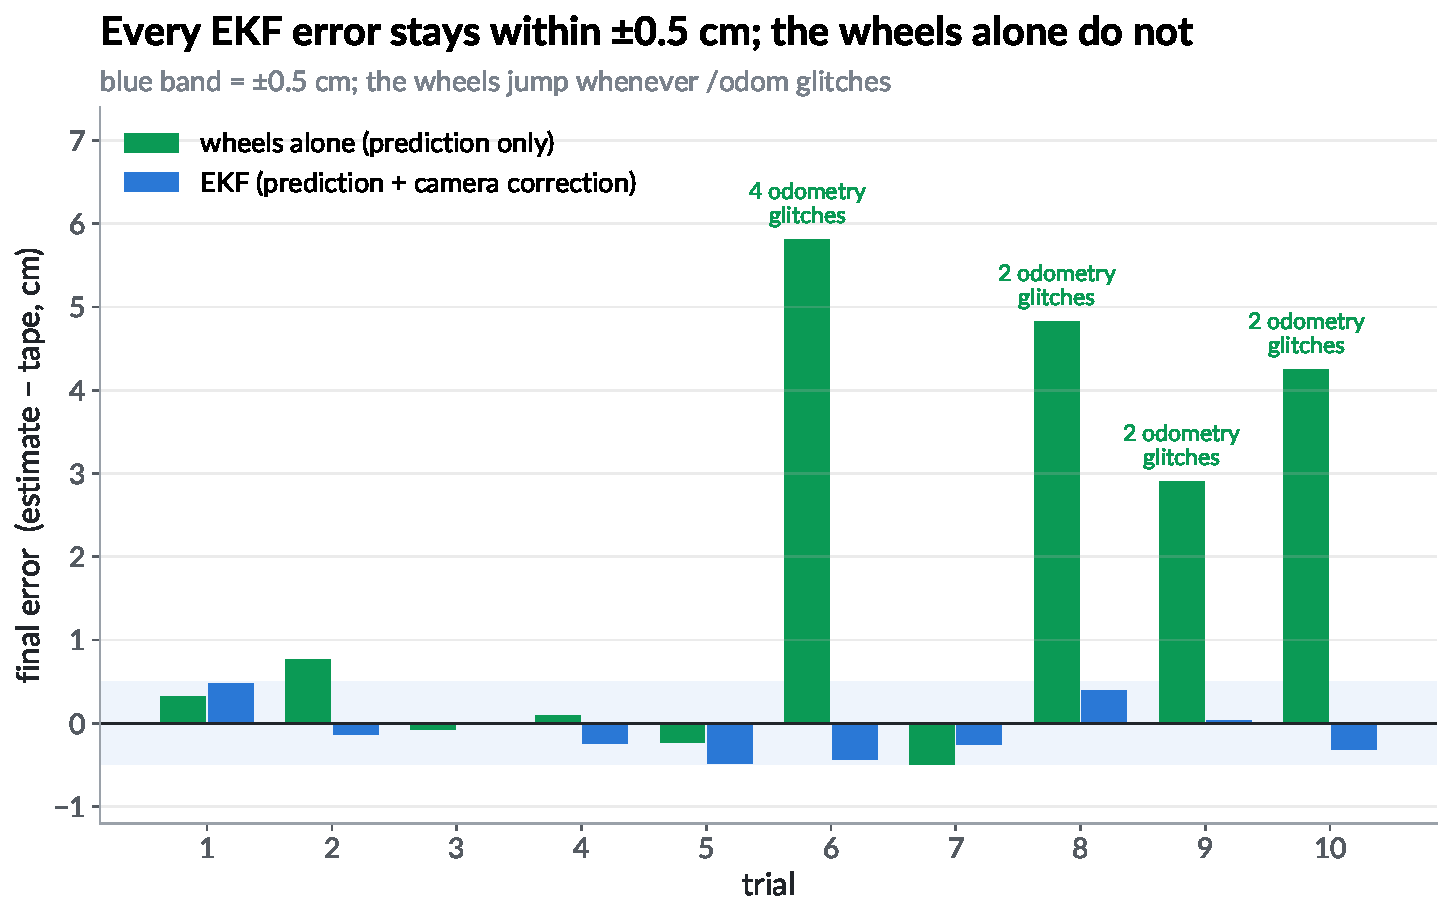
\includegraphics[width=0.92\linewidth]{figures/simple_2_per_trial.pdf}
\caption{Final error of every trial for the EKF (blue) and for the wheels alone (green).
\textbf{How to read it:} the closer a bar is to zero, the better. The EKF bars all stay in the $\pm$0.5\,cm band.
The wheels alone are as good in trials 1 to 5 and 7, but jump to 2.9 to 5.8\,cm in the four trials in which \code{/odom}
glitched: odometry has no way to notice its own error, the camera correction does.}
\label{fig:errors}
\end{figure}

%-----------------------------------------------------------------------------
\isub{\faCalculator}{Statistical analysis}
\label{sec:stats}
With $N=10$ trials and $e_i = d_{est,i}-d_{meas,i}$:
\begin{equation}
\text{MAE}=\frac1N\sum_{i=1}^{N}|e_i|,\quad \text{range}=\max_i e_i-\min_i e_i,\quad
\bar e=\frac1N\sum e_i,\quad s=\sqrt{\tfrac{1}{N-1}\textstyle\sum (e_i-\bar e)^2},\quad
\text{RMSE}=\sqrt{\tfrac1N\textstyle\sum e_i^2}.
\end{equation}

\begin{table}[H]
\centering\small
\setlength{\tabcolsep}{6pt}
\rowcolors{2}{kfupmlight}{white}
\begin{tabular}{@{}lrrrrrr@{}}
\rowcolor{kfupm}\hd{Method} & \hd{MAE} & \hd{bias $\bar e$} & \hd{std.\ dev.\ $s$} & \hd{RMSE} & \hd{min / max} & \hd{range}\\
\textbf{EKF (predict + correct)} & \textbf{0.28} & $-0.10$ & 0.32 & 0.32 & $-0.48$ / $+0.48$ & \textbf{0.96}\\
Camera alone & 0.29 & $-0.16$ & 0.30 & 0.33 & $-0.54$ / $+0.40$ & 0.95\\
Wheels alone & 1.98 & $+1.81$ & 2.39 & 2.91 & $-0.50$ / $+5.81$ & 6.31\\
\end{tabular}
\caption{Descriptive statistics of the final error, in cm.}
\label{tab:descr}
\end{table}

\begin{figure}[H]
\centering
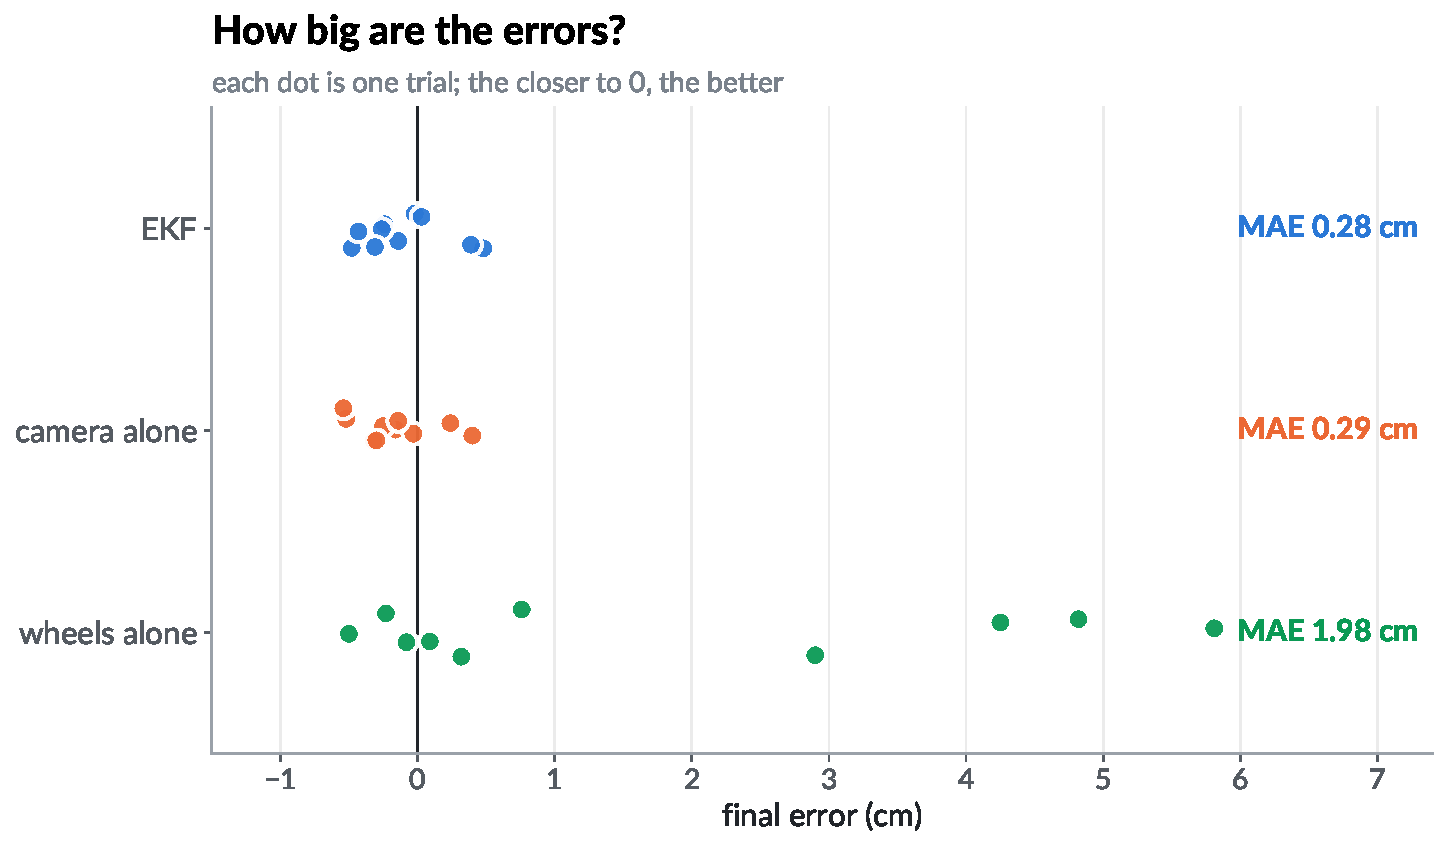
\includegraphics[width=0.84\linewidth]{figures/simple_3_spread.pdf}
\caption{All 30 errors on one axis. \textbf{How to read it:} each dot is a trial; a tight cluster around zero means an
accurate and repeatable method. The EKF and the camera form a tight cluster within half a centimetre; the wheels alone
spread over six centimetres.}
\label{fig:spread}
\end{figure}

\lead{Is there a systematic error (bias)?} A one-sample $t$-test of $H_0: \bar e = 0$ gives $t=-0.96$, $p=0.36$ for
the EKF; the 95\,\% confidence interval of the mean error is $[-0.33,\ +0.13]$\,cm and contains zero. \emph{The EKF has no
detectable bias.} The wheels alone have a significant bias of $+1.81$\,cm ($t=2.40$, $p=0.04$, interval
$[+0.10,\ +3.53]$\,cm): when odometry steps are lost, the wheels under-count the travel and think the robot is farther from
the tag than it is.

\lead{Does the estimate follow reality?} A least-squares fit of $d_{est}$ on $d_{meas}$ gives a slope of
$0.99 \pm 0.17$ (standard error), an intercept of 0.23\,cm and $R^2=0.81$ ($p=0.0004$); the Pearson correlation is
$r=0.90$ and the covariance $\operatorname{cov}(d_{est},d_{meas})=0.445$\,cm$^2$. A slope of one means that when the robot
really stops 1\,cm earlier, the estimate also says 1\,cm earlier.

\lead{Is the EKF better than the wheels alone?} In spread, clearly: the variance ratio is
$F = s^2_{wheels}/s^2_{EKF} = 54.6$ ($p<0.001$; Levene's test $p=0.013$). In absolute error the Wilcoxon signed-rank test
gives $p=0.084$: with ten trials and odometry already good in six of them, the difference in \emph{typical} error is not
significant at 5\,\%, while the difference in \emph{reliability} (worst case 0.48 against 5.81\,cm) is. Against the camera
alone the EKF is not different ($p=0.38$), as expected when the camera sees the tag until the stop
(Section~\ref{sec:role}). The EKF errors are compatible with a normal distribution (Shapiro--Wilk $p=0.28$).

\begin{figure}[H]
\centering
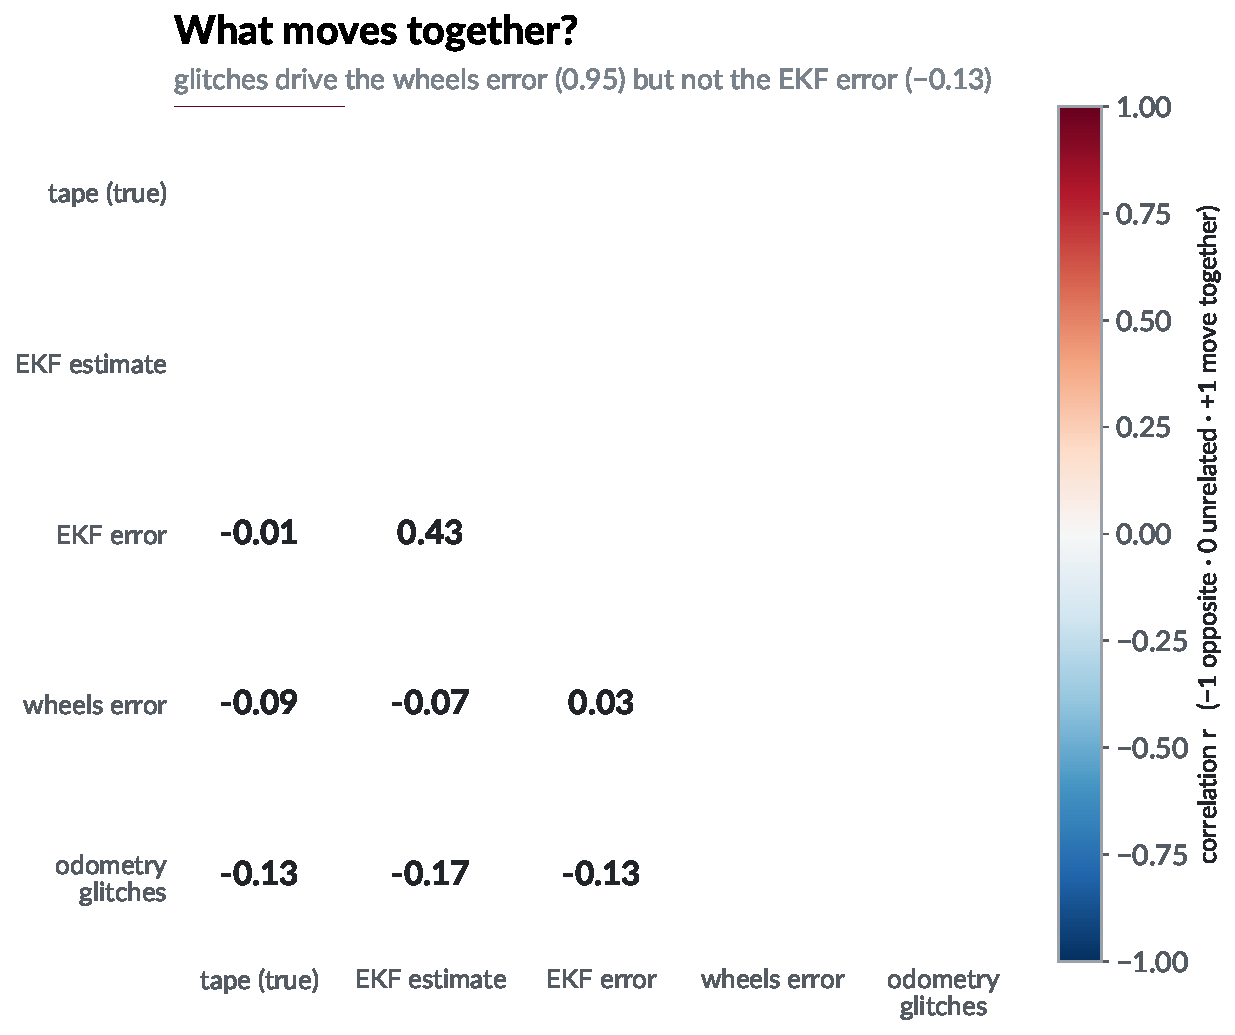
\includegraphics[width=0.70\linewidth]{figures/simple_4_correlation.pdf}
\caption{Correlation matrix of five per-trial quantities. \textbf{How to read it:} $+1$ means two quantities rise
together, 0 means unrelated. Three cells tell the story: estimate and tape move together (0.90); the wheels error is
driven by the odometry glitches (0.95); the EKF error is not ($-0.13$), because the camera correction removes what the
glitches add.}
\label{fig:corr}
\end{figure}

\begin{figure}[H]
\centering
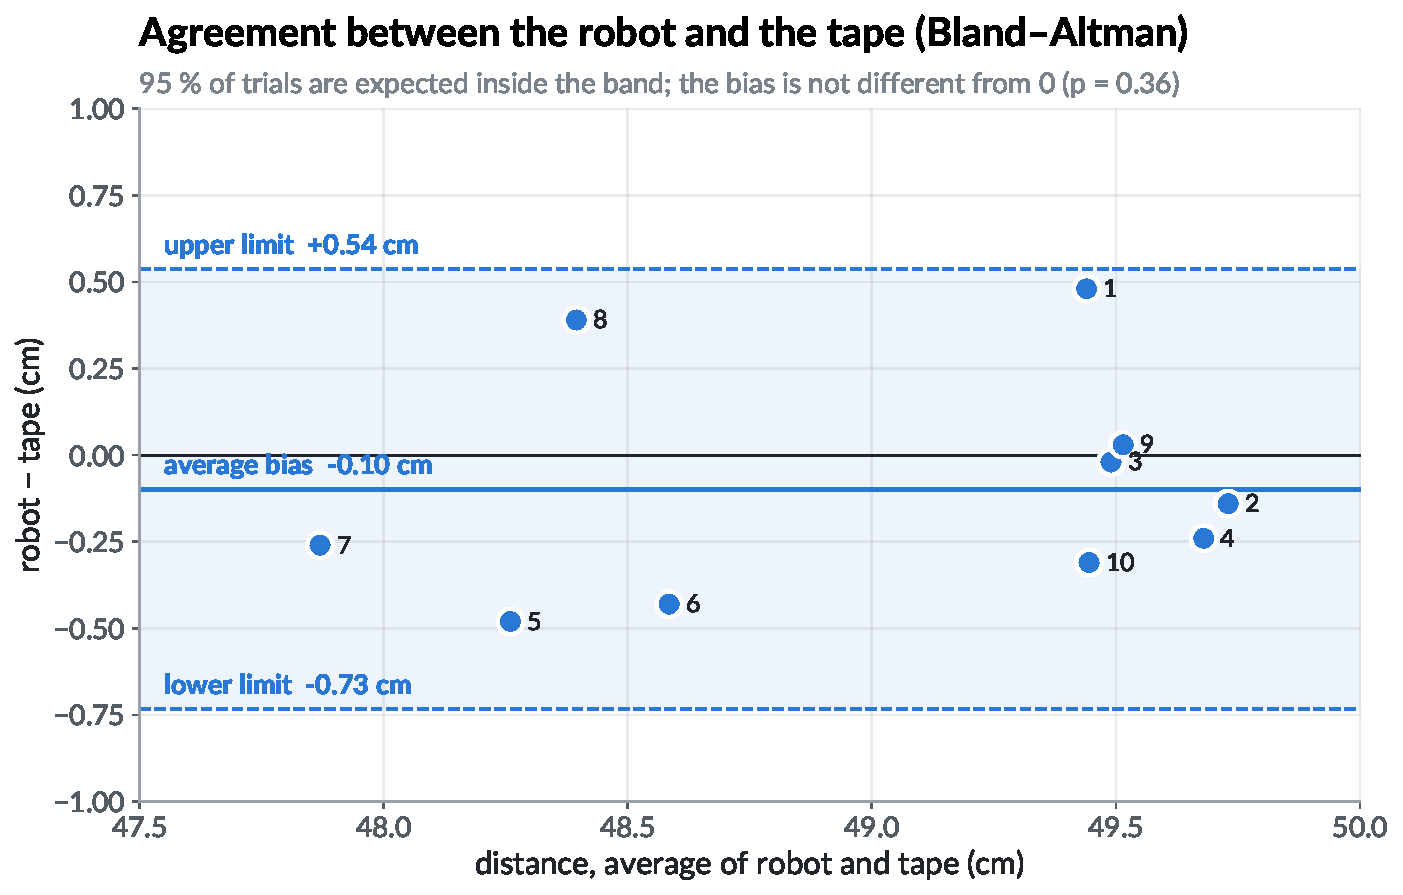
\includegraphics[width=0.84\linewidth]{figures/simple_5_agreement.pdf}
\caption{Bland--Altman plot, the standard way to compare two methods that measure the same quantity.
\textbf{How to read it:} each dot is a trial, the vertical axis is how far the robot is from the tape. The solid line is
the average bias ($-0.10$\,cm) and the dashed lines are the 95\,\% limits of agreement, $-0.73$ to $+0.54$\,cm: a new
trial is expected to agree with the tape within this band. The differences do not grow with the distance, so there is no
scale error.}
\label{fig:ba}
\end{figure}

\begin{notebox}
\small\lead{Why no confusion matrix?} A confusion matrix counts right and wrong \emph{class} decisions. This experiment
measures a continuous distance, so agreement is assessed with the scatter plot and regression, the Bland--Altman
limits of agreement and the correlation matrix above.
\end{notebox}

%-----------------------------------------------------------------------------
\isub{\faChartLine}{During the drive}
\begin{figure}[H]
\centering
\begin{subfigure}[t]{0.49\linewidth}\centering
  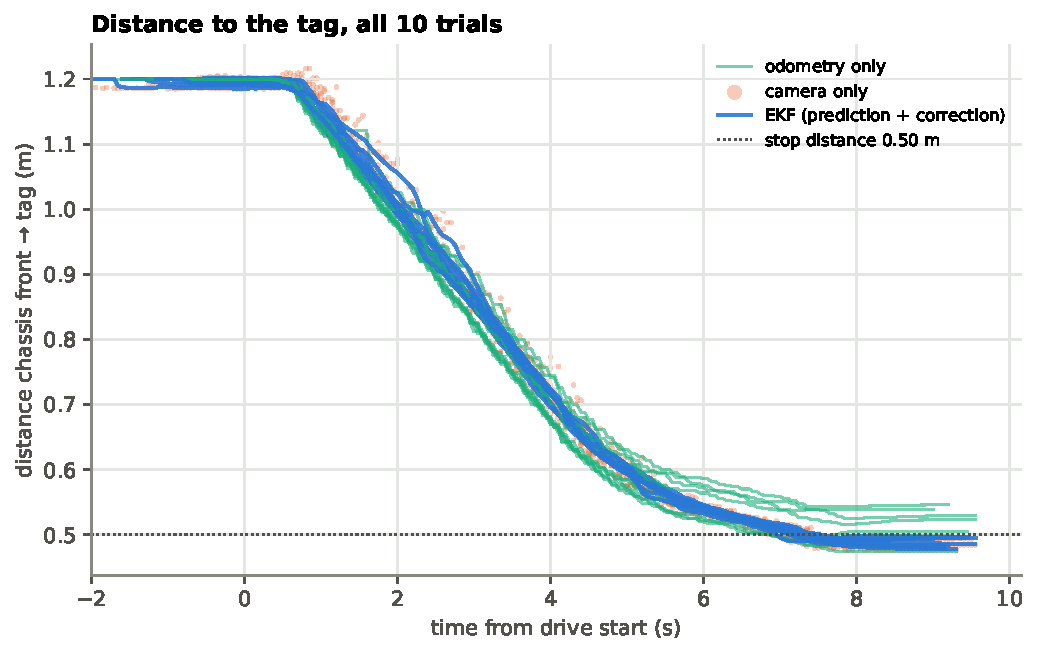
\includegraphics[width=\linewidth]{figures/fig3_distance_vs_time.pdf}
  \caption{Distance to the tag during every trial.}
  \label{fig:dist}
\end{subfigure}\hfill
\begin{subfigure}[t]{0.49\linewidth}\centering
  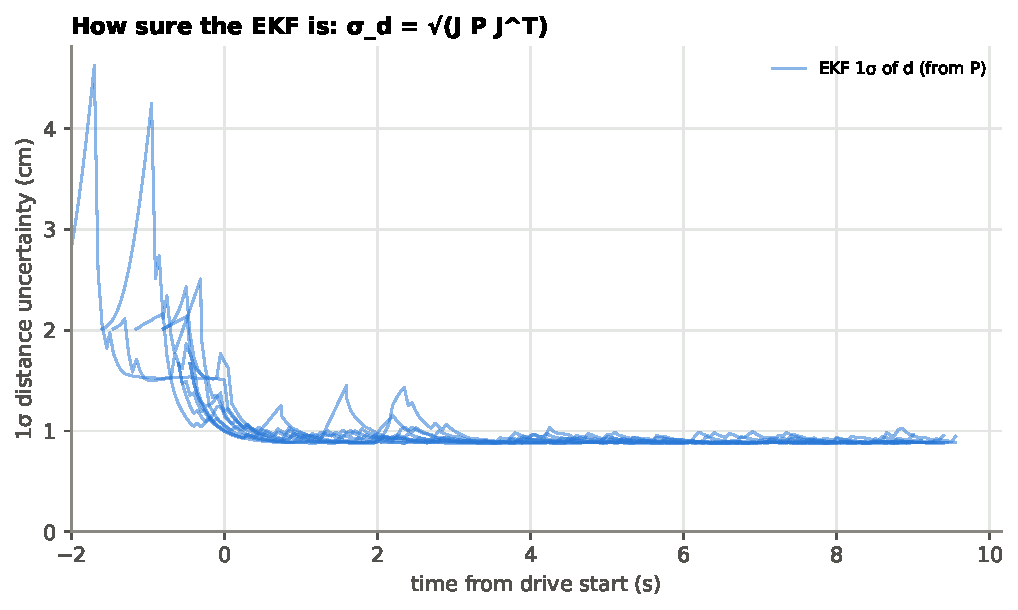
\includegraphics[width=\linewidth]{figures/fig4_ekf_uncertainty.pdf}
  \caption{EKF uncertainty $\sigma_d$ during every trial.}
  \label{fig:sigma}
\end{subfigure}
\caption{Time histories. The uncertainty starts at the placement accuracy, drops as soon as the camera fixes arrive,
and stays below 1\,cm while driving because a camera correction arrives every 70\,ms on average.}
\label{fig:stats}
\end{figure}

\begin{figure}[H]
\centering
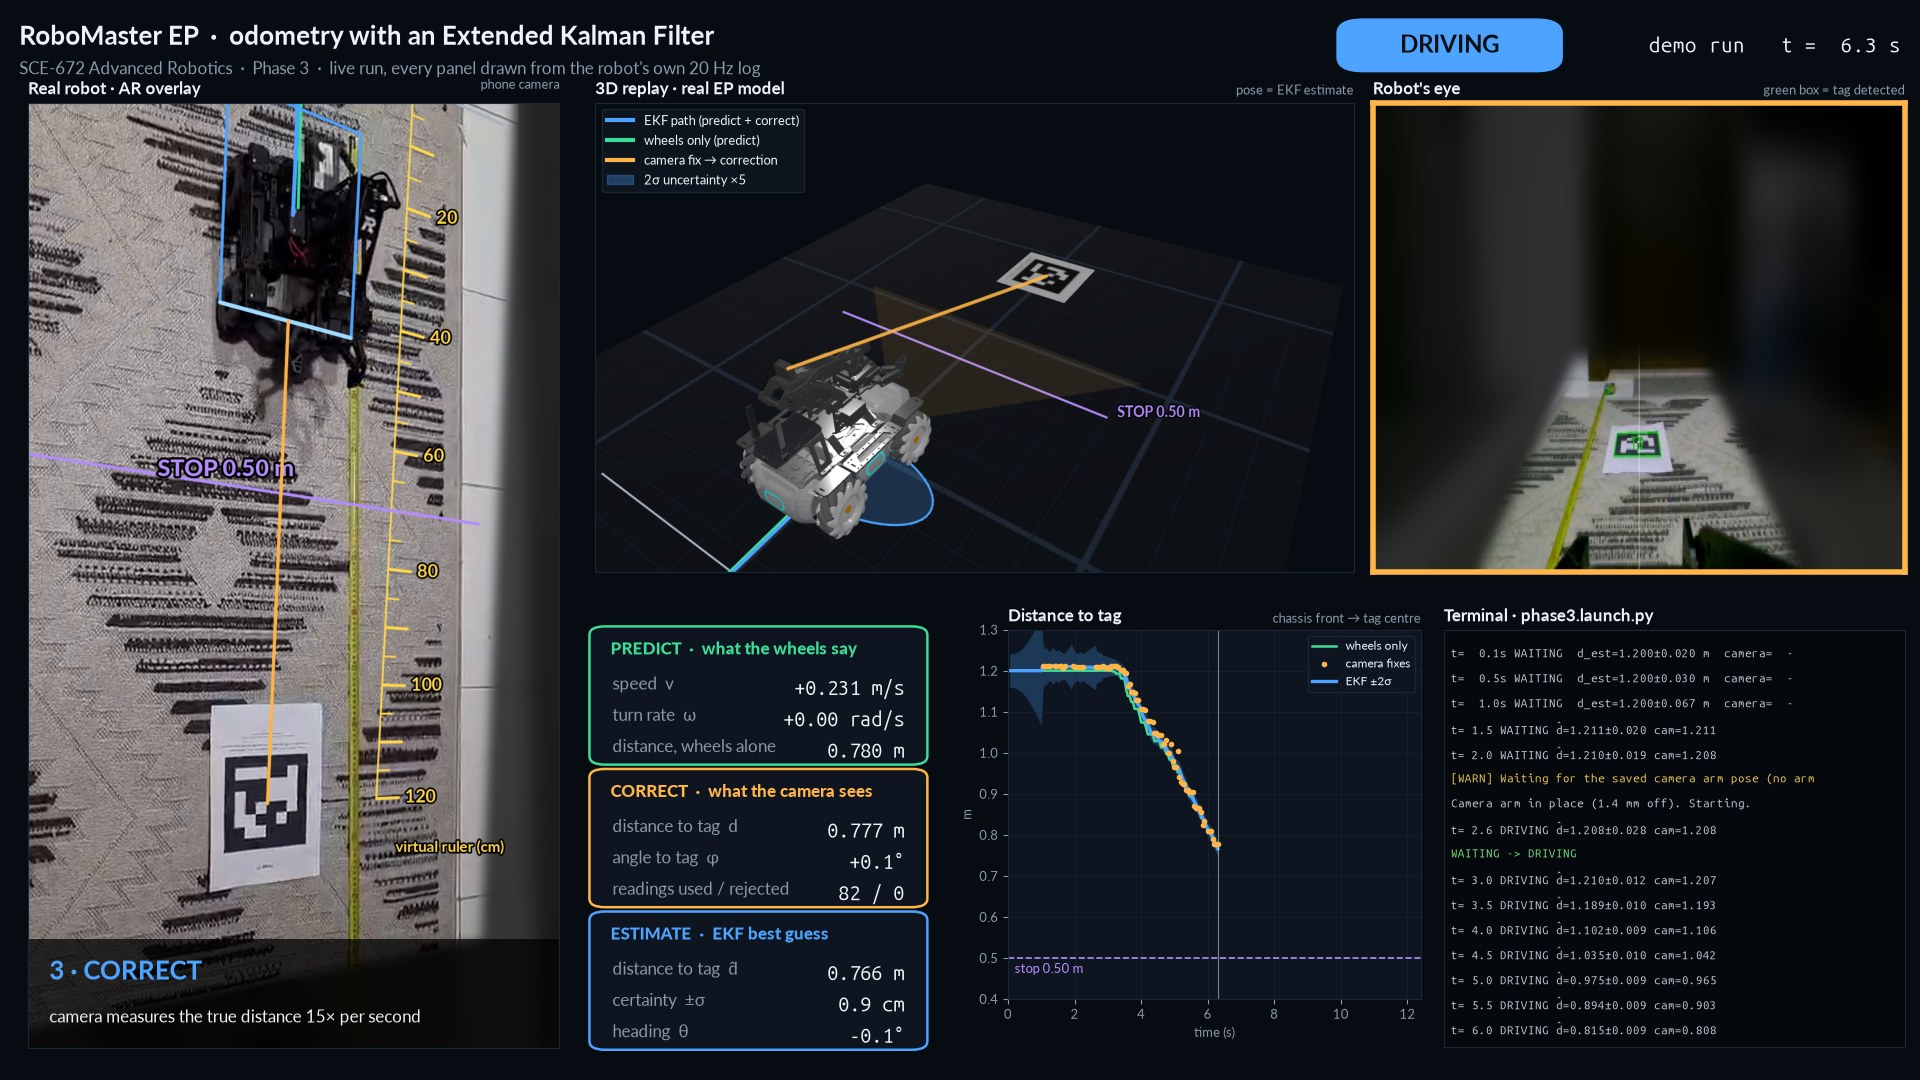
\includegraphics[width=\linewidth]{figures/still_driving.jpg}
\caption{Frame of the demo video (\link{\videolink}{link}). Left: phone video with an augmented-reality overlay drawn
on the floor from the tag's own pose (blue outline: the EKF estimate of the robot footprint; yellow: virtual ruler
next to the real tape; orange: the current camera correction). Right: 3D replay with DJI's EP model, the robot's camera,
the three groups of numbers, the distance history and the terminal.}
\label{fig:video}
\end{figure}
